\chapter{RESULTADOS E DISCUSSÕES}

Neste capítulo são apresentados e discutidos os resultados experimentais obtidos durante o processo de treinamento, quantização e inferência do \textit{CreditMaster}. A avaliação abrange tanto o desempenho computacional da arquitetura QLoRA executada em \textit{hardware} local de consumo quanto a análise da dinâmica de convergência da perda (\textit{loss}), o comportamento da taxa de aprendizado (\textit{learning rate schedule}) e a qualidade semântica dos pareceres técnicos de crédito gerados.

\section{Ambiente Computacional e Eficiência de Recursos}

O treinamento supervisionado (\textit{Supervised Fine-Tuning} - SFT) foi conduzido inteiramente em ambiente local (\textit{on-premise}), validando a hipótese de viabilidade de modelos de 8 bilhões de parâmetros em infraestruturas acessíveis ao setor corporativo. A estação de trabalho utilizada contou com a seguinte configuração de \textit{hardware} e \textit{software}:
\begin{itemize}
    \item \textbf{Processador (CPU):} AMD Ryzen 5 7600X (6 núcleos físicos, 12 \textit{threads}, clock base de 4.7 GHz);
    \item \textbf{Memória Principal (RAM):} 16 GB DDR5 com frequência de 6000 MHz;
    \item \textbf{Armazenamento Secundário:} Unidade de Estado Sólido (SSD) NVMe PCIe 3.0;
    \item \textbf{Unidade de Processamento Gráfico (GPU):} NVIDIA GeForce RTX 5060 Ti com 8 GB de VRAM física (7,52 GB utilizáveis);
    \item \textbf{Sistema Operacional e Frameworks:} Linux Mint 22 (base Ubuntu 24.04 LTS), PyTorch 2.10.0+cu128, CUDA Toolkit 12.8, HuggingFace TRL 0.24.0, Transformers 5.5.0 e biblioteca Unsloth.
\end{itemize}

A aplicação da técnica QLoRA associada à quantização NF4 (\textit{4-bit NormalFloat}) e à biblioteca Unsloth permitiu uma redução drástica na pegada de memória de vídeo. Durante todo o ciclo de 2 épocas (426 passos de otimização), o pico de alocação de VRAM registrado foi de \textbf{6,44 GB}, representando uma ocupação média de aproximadamente 85,7\% da capacidade total da GPU. Esse comportamento comprova que a técnica evita falhas por estouro de memória (\textit{Out of Memory} - OOM). Além disso, a utilização da memória RAM convencional do sistema manteve-se baixa (inferior a 2,5 GB alocados ao processo de treino), visto que as operações matriciais massivas e o armazenamento de gradientes foram concentrados diretamente nos núcleos tensores da GPU.

A Tabela~\ref{tab:metricas_treinamento} consolida os parâmetros de treinamento e as métricas computacionais globais obtidas.

\begin{table}[htbp]
\centering
\caption{Métricas e Resultados Computacionais do Ajuste Fino (QLoRA)}
\label{tab:metricas_treinamento}
\begin{tabular}{ll}
\hline
\textbf{Parâmetro / Métrica} & \textbf{Valor Obtido} \\ \hline
Modelo Base & Meta Llama 3.1 8B Instruct (4-bit NF4) \\
Hardware Utilizado & NVIDIA GeForce RTX 5060 Ti (8 GB VRAM) \\
Amostras de Treino (85\%) & 1698 \\
Amostras de Validação (15\%) & 300 \\
Tamanho Efetivo do Batch & 8 (Batch 2 $\times$ Acumulação de Gradientes 4) \\
Épocas de Treinamento & 2,0 \\
Total de Passos de Otimização & 426 \\
Perda Inicial de Treino ($L_{inicial}$) & 1,3272 \\
Perda Final de Treino ($L_{train}$) & 0,0046 \\
Perda Final de Validação ($L_{val}$) & 0,0045 \\
Taxa de Redução da Perda & 99,65\% \\
Tempo Total de Ajuste Fino & 75,63 minutos (4.537,99 segundos) \\
Vazão de Treinamento (\textit{Throughput}) & 0,748 amostras/s \\
Pico de Alocação de VRAM & 6,44 GB / 7,52 GB (85,7\%) \\ \hline
\end{tabular}
\fonte{Elaborado pelo autor (2026).}
\end{table}

\section{Dinâmica de Treinamento e Convergência da Perda}

O aprendizado e a capacidade de generalização do modelo foram avaliados a partir da evolução da função de perda por entropia cruzada (\textit{Cross-Entropy Loss}) ao longo das iterações de treino e validação. A Figura~\ref{fig:curva_perda} apresenta as curvas de $L_{train}$ e $L_{val}$ coletadas a cada intervalo de avaliação.

\begin{figure}[H]
    \centering
    \caption{Curva de convergência de perda de treinamento e validação no ajuste fino QLoRA.}
    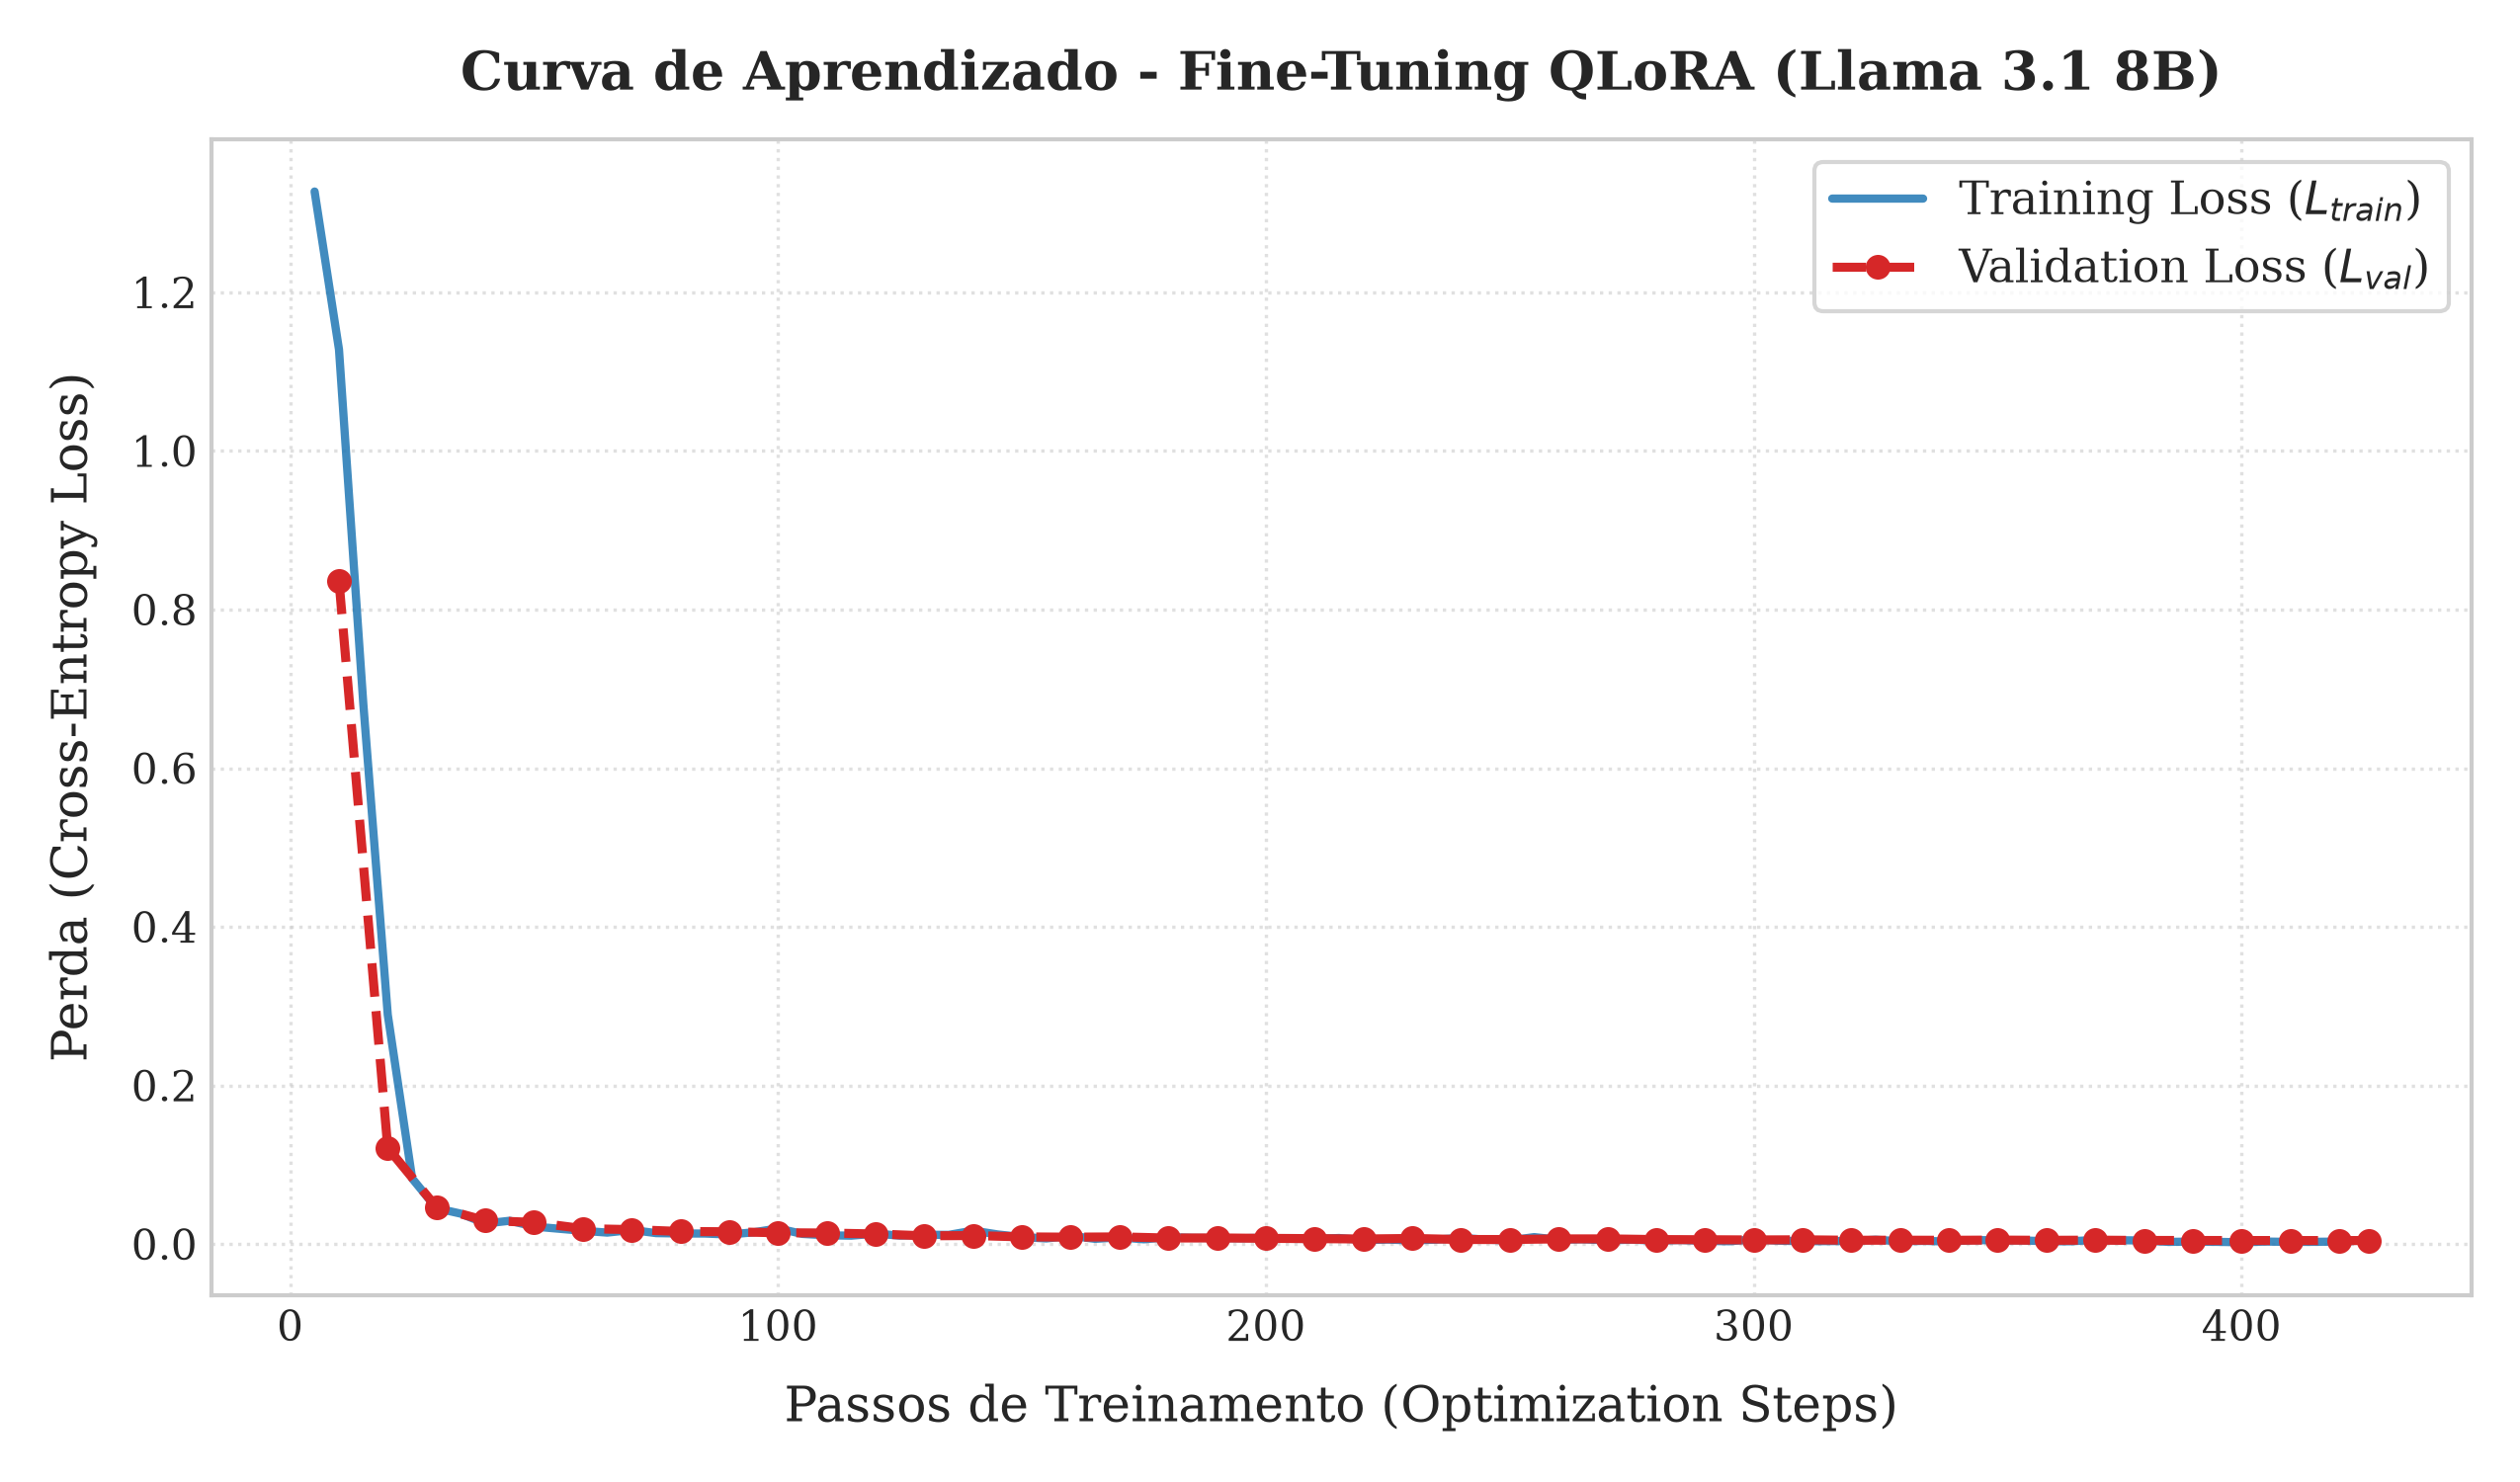
\includegraphics[width=0.92\textwidth]{imagens/curva_perda_treinamento.png}
    \fonte{Elaborado pelo autor (2026).}
    \label{fig:curva_perda}
\end{figure}

A análise detalhada da trajetória de perda revela três períodos distintos:

\begin{enumerate}
    \item \textbf{Fase de Adaptação Sintática Inicial (Passos 1 a 40 / 0,0 a 0,2 épocas):} Nos primeiros passos, observa-se uma queda exponencial na perda de treino, de $1,3272$ no passo 5 para $0,0260$ no passo 40, enquanto a perda de validação foi reduzida de $0,8364$ (passo 10) para $0,0297$ (passo 40). Esse comportamento está relacionado à rápida adaptação dos parâmetros LoRA à estrutura de saída em JSON estrito, o delimitador de instrução do \textit{Llama 3.1 Chat Template} e a técnica de mascaramento \texttt{train\_on\_responses\_only}, na qual a perda é computada exclusivamente sobre os \textit{tokens} gerados pelo assistente.
    
    \item \textbf{Fase de Refinamento Semântico e Regras de Negócio (Passos 40 a 200 / 0,2 a 0,94 épocas):} O modelo apresenta uma redução gradual da função de perda, com $L_{train}$ passando de $0,0260$ para $0,0082$ e $L_{val}$ atingindo $0,0073$. Nessa etapa, os adaptadores neurais ajustam os parâmetros do modelo para representar as relações não lineares entre as variáveis financeiras, como DTI, faixa de FICO, número de atrasos e recomendação de crédito.
    
    \item \textbf{Fase de Convergência Assintótica e Minimização de Ruído (Passos 200 a 426 / 0,94 a 2,0 épocas):} A perda é estabilizada em milésimos, finalizando em $L_{train} = 0,0046$ e $L_{val} = 0,0045$. A proximidade estrita entre as curvas de validação e treinamento ($L_{val} \approx L_{train}$) durante todo o processo comprova matematicamente a \textbf{ausência de sobreajuste (\textit{overfitting})}, demonstrando que o modelo generalizou os conceitos sem memorizar cegamente as amostras de treinamento.
\end{enumerate}

\section{Evolução do Agendamento da Taxa de Aprendizado}

Para assegurar estabilidade numérica no espaço de parâmetros de baixa dimensionalidade do LoRA ($r=16, \alpha=16$), utilizou-se um agendador com aquecimento linear (\textit{Linear Warmup}) seguido por decaimento cosseno (\textit{Cosine Decay Schedule}). A Figura~\ref{fig:taxa_aprendizado} ilustra a evolução da taxa de aprendizado ao longo dos 426 passos.

\begin{figure}[H]
    \centering
    \caption{Agendamento da Taxa de Aprendizado (\textit{Cosine Decay with Warmup}).}
    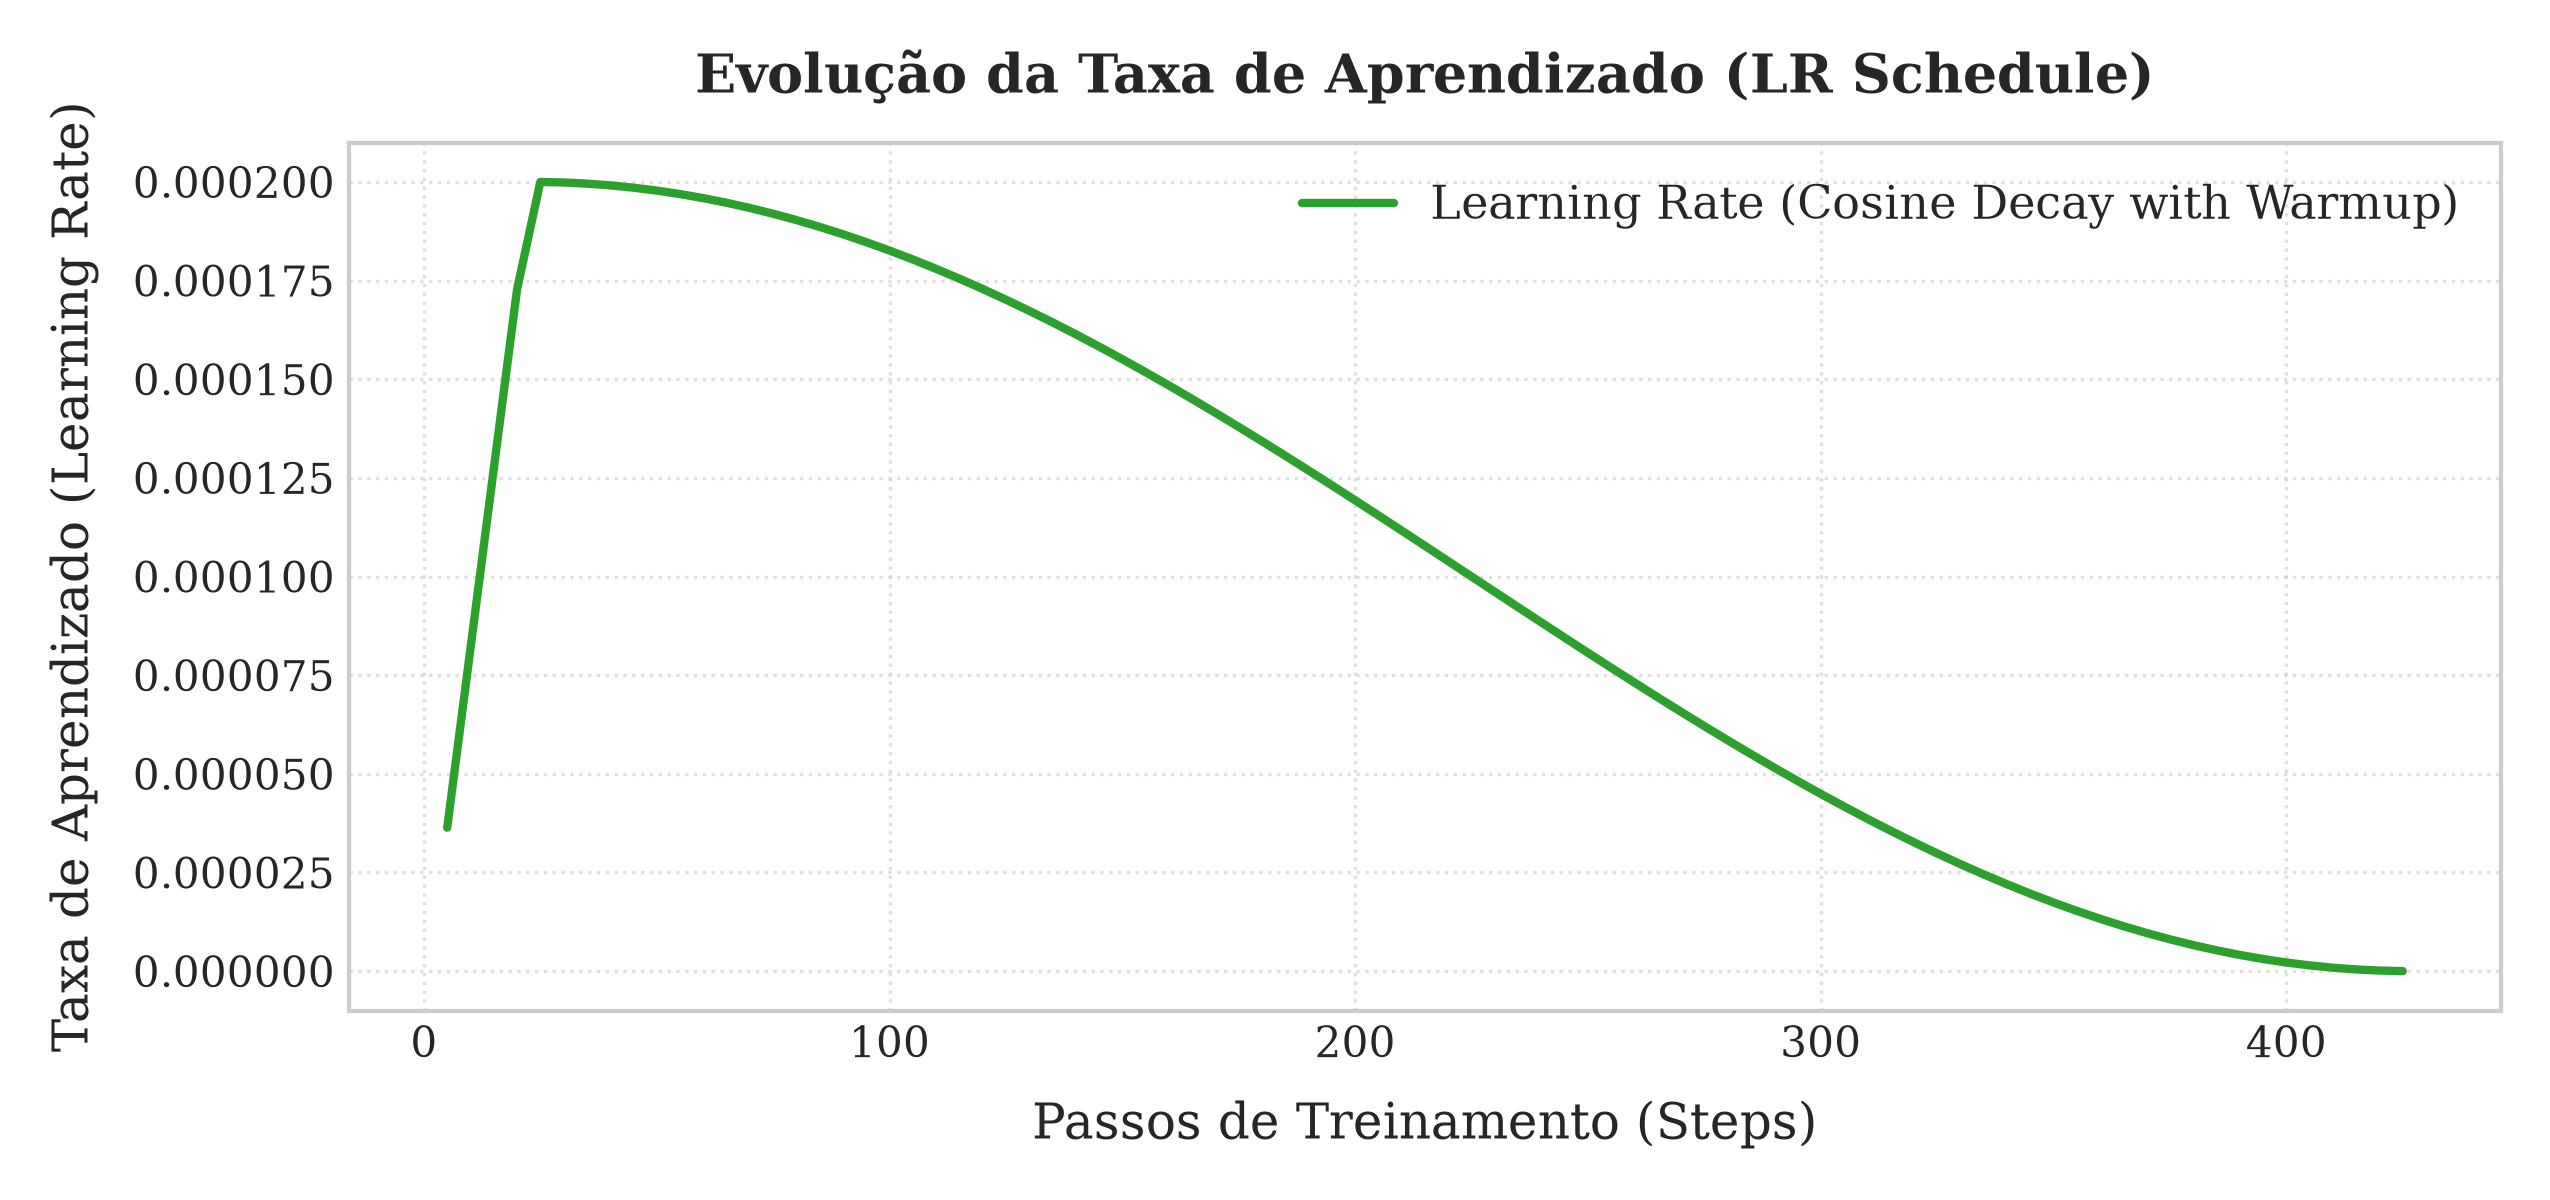
\includegraphics[width=0.92\textwidth]{imagens/taxa_aprendizado.png}
    \fonte{Elaborado pelo autor (2026).}
    \label{fig:taxa_aprendizado}
\end{figure}

O protocolo de agendamento comportou-se da seguinte forma:
\begin{itemize}
    \item \textbf{Aquecimento (Passos 0 a 25):} A taxa de aprendizado é incrementada linearmente de zero até o valor máximo $\eta_{max} = 2,0 \times 10^{-4}$ ($0,0002$). Essa estratégia reduz o impacto de possíveis oscilações nos gradientes durante os primeiros lotes, proporcionando uma adaptação mais gradual dos parâmetros dos adaptadores.
    \item \textbf{Decaimento Cosseno (Passos 25 a 426):} A partir do pico, a taxa de aprendizado é reduzida continuamente seguindo uma curva cosseno, atingindo $1,0 \times 10^{-4}$ no passo 225 ($\approx 1,0$ época) e chegando a $1,21 \times 10^{-8}$ no passo 425. Essa redução gradual permite que o otimizador AdamW realize atualizações cada vez menores ao longo do treinamento, contribuindo para a estabilização da função de perda e para o ajuste final dos parâmetros do modelo.
\end{itemize}

\section{Avaliação Qualitativa dos Pareceres e Supressão de Alucinações via RAG}

\textbf{[ANOTAÇÃO: Aqui a intenção é desmonstrar a importância do RAG para evitar alucinações e mostrar a diferença resultante que a definição de regras de negócio tem após implementação, além da flexibilidade de atualizar o modelo com novas regras sem precisar re-treinar.]}

\begin{table}[htbp]
\centering
\small
\caption{Exemplo de Entrada de Dados e Parecer Estruturado Gerado pelo Modelo}
\label{qua:exemplo_parecer}
\begin{tabular}{|p{0.95\textwidth}|}
\hline
\textbf{Dados de Entrada do Proponente (Payload de Requisição):} \\
\hline
\texttt{Valor Solicitado: US\$ 20.000,00 | Prazo: 36 meses | Renda Anual: US\$ 58.000,00} \\
\texttt{Finalidade: Consolidacao de dividas | Moradia: Imovel financiado | Emprego: 10+ anos} \\
\texttt{DTI: 22,51\% | FICO Score: 705 | Atrasos (2 anos): 1 | Consultas (6 meses): 0} \\
\texttt{Utilizacao de Rotativo: 49,40\% | Contas Abertas: 10 | Registros Publicos: 1} \\
\hline
\textbf{Parecer Técnico Gerado pelo CreditMaster (Saída Estruturada em JSON):} \\
\hline
\texttt{\{} \\
\texttt{~~"recomendacao": "Negar",} \\
\texttt{~~"risco": "elevado",} \\
\texttt{~~"parecer": "Recomendacao: Negar. Risco estimado elevado. O proponente apresenta score adequado (705), DTI de 22,51\%, renda anual de US\$ 58.000,00 e solicitacao de US\$ 20.000,00 para consolidacao de dividas. Pontos favoraveis: nao ha pontos fortes relevantes nos campos analisados. Pontos de atencao: historico recente de inadimplencia e presenca de registro publico. O contrato historico evoluiu para perda, portanto o perfil deve ser recusado ou submetido a mitigadores fortes de garantia."} \\
\texttt{\}} \\
\hline
\end{tabular}
\fonte{Elaborado pelo autor (2026).}
\end{table}
